\documentclass{beamer}
\mode<presentation>
\usetheme{CambridgeUS}
\usecolortheme{beaver}

\usepackage[english]{babel}
\usepackage{graphicx}
\usepackage{subfigure}
\usepackage{url}
\usepackage[backend=bibtex, style=verbose]{biblatex}
\bibliography{bibliography.bib}
\usepackage[noend]{algorithm,algpseudocode}


\title[Dynamic Routing Between Capsules]{Dynamic Routing Between Capsules}
\author[Mu\c sat Bogdan-Adrian]{Authors: Sara Sabour, Nicholas Frosst, Geoffrey E Hinton}
\date{November 2017}

\beamertemplatenavigationsymbolsempty
\graphicspath{{./images/}}

\begin{document}

\frame{\titlepage}

\begin{frame}
\frametitle{Introduction}
\center
\begin{itemize}
	\item A capsule is a group of neurons whose activity vector represents an entity - either an object or an object part
	\item The length of the vector represents the probability that a certain entity exists
	\item Achieves state-of-the-art performance on MNIST and is better at recognizing highly overlapping digits than a convolutional network
\end{itemize}
\end{frame}

\begin{frame}
\frametitle{Reference with human vision}
\center
\begin{itemize}
	\item The human vision processes only a tiny fraction of the optic array at the highest resolution
	\item Assumption that the visual system creates a parse tree on each fixation
	\begin{figure}
	\subcapcentertrue
    \centering
    	\subfigure[Parse tree example: \newline (7 + 3) * (5 - 2)]
        {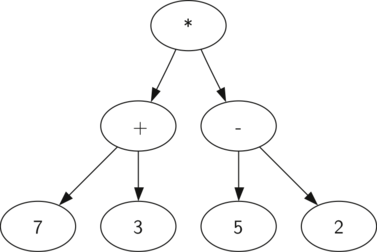
\includegraphics[width=0.4\textwidth]{parse_tree.png}}
    \end{figure}
\end{itemize}
\end{frame}

\begin{frame}
\frametitle{Capsules as parse trees}
\center
\begin{itemize}
	\item A parse tree can be represented by a multilayer neural network
	\item Each layer will be divided into many capsules
	\item Using an iterative routing process, each capsule will choose a capsule in the layer above to be its parent in the tree - this process solves the problem of assigning parts to wholes
\end{itemize}
\end{frame}

\begin{frame}
\frametitle{Describing the capsule}
\center
\begin{itemize}
	\item The vector of activities of a capsule represent the various properties of a particular entity that is present in the image (pose, deformation, velocity, texture etc.)
	\item The existence of an object is defined by using the overall length of the activity vector of a capsule - a non-linearity is applied so that the length of the vector output cannot exceed 1
	\item A lower level capsule is assigned to a higher level capsule by a ``routing-by-agreement'' algorithm
\end{itemize}
\end{frame}

\begin{frame}
\frametitle{How the vector inputs and outputs of a capsule are computed}
The length of the output vector of a capsule should represent the probability that the entity represented by the capsule is present in the current input. A non-linear squashing function is used to ensure that short vectors get shrunk to almost zero length and long vectors get shrunk to a length slightly below 0:
\begin{equation}
\begin{split}
v_j = \frac{\lVert s_j \rVert^2}{1 + \lVert s_j \rVert^2} \frac{s_j}{\lVert s_j \rVert^2}
\end{split}
\end{equation}
where \(v_j\) is the vector output of capsule \(j\) and \(s_j\) is its total input.
\end{frame}

\begin{frame}
\frametitle{How the vector inputs and outputs of a capsule are computed}
For all but the first layer of capsules, the total input to a capsule \(s_j\) is a weighted sum over all prediction vectors \(\hat{u}_{j|i}\) from the capsules in the layer below and is produced by multiplying the output \(u_i\) of a capsule in the layer below by a weight matrix \(W_{ij}\):
\begin{equation}
\begin{split}
s_j = \sum_{i}c_{ij}\hat{u}_{i|j}, \ \ \ \hat{u}_{i|j} = W_{ij}u_i
\end{split}
\end{equation}
where the \(c_{ij}\) are coupling coefficients that are determined by the iterative dynamic routing process.
\end{frame}

\begin{frame}
\frametitle{How the vector inputs and outputs of a capsule are computed}
The coupling coefficients between capsule i and all the capsules in the layer above sum to 1 and are determined by a ``routing softmax'' whose initial logits \(b_{ij}\) are the log prior probabilities that capsule \(i\) should be coupled to capsule \(j\):
\begin{equation}
\begin{split}
c_{ij} = \frac{exp(b_{ij})}{\sum_{k}exp(b_{ik})}
\end{split}
\end{equation}
The initial coupling coefficients are iteratively refined by measuring the agreement between the current output \(v_j\) of each capsule, \(j\), in the layer above and the prediction \(\hat{u}_{j|i}\) made by capsule \(i\).
\end{frame}

\begin{frame}
\frametitle{How the vector inputs and outputs of a capsule are computed}
The agreement is simply the scalar product \(a_{ij} = v_j \cdot \hat{u}_{j|i}\). This agreement is treated as if it were a log likelihood and is added to the initial logit, \(b_{ij}\) before computing the new values for all the coupling coefficients linking capsule \(i\) to higher level capsules.
\end{frame}

\begin{frame}
\frametitle{Routing algorithm}
\begin{algorithmic}[1]
\Function{ROUTING}{$\hat{u}_{j|i}, r, l$}
	\State for all capsule $i$ in layer $l$ and capsule $j$ in layer ($l$ + 1): $b_{ij} \gets$ 0.
		\For {$r$ iterations}
			\State for all capsule $i$ in layer $l$: $c_i \gets$ softmax($b_i$)
			\State for all capsule $j$ in layer ($l$ + 1): $s_j \gets \sum_{i}c_{ij}\hat{u}_{j|i}$
			\State for all capsule $j$ in layer ($l$ + 1): $v_j \gets$ squash($s_j$)
			\State for all capsule $i$ in layer $l$ and capsule $j$ in layer ($l$ + 1): 
			\State \ \ \ \ $b_{ij} \gets b_{ij} + \hat{u}_{j|i} \cdot v_j$
		\EndFor
		\Return $v_j$
\EndFunction
\end{algorithmic}
\end{frame}

\begin{frame}
\frametitle{Margin loss for digit existence}
Because the length of the instantiation vector is used to represent the probability that a capsule's entity exists, the top-level capsule for digit class k should have a long vector if and only if that digit is present in the image. For multiple digits, a margin loss is used:
\begin{equation}
\begin{split}
L_c = T_c max(0, m^+ - \lVert v_c \rVert)^2 + \lambda (1 - T_c) max(0, \lvert v_c \rVert - m^-)^2
\end{split}
\end{equation}
where \(T_c = 1\) iff a digit of class \(c\) is present and \(m^+ = 0.9\) and \(m^- = 0.1\). The \(\lambda\) down-weighting of the loss for absent digit classes stops the initial learning from shrinking the lengths of the activity vectors of all the digit capsules. The total loss is simply the sum of the losses of all digit capsules.
\end{frame}

\begin{frame}
\frametitle{CapsNet architecture}
\begin{figure}
	\subcapcentertrue
    \centering
    	\subfigure[CapsNet architecture]
        {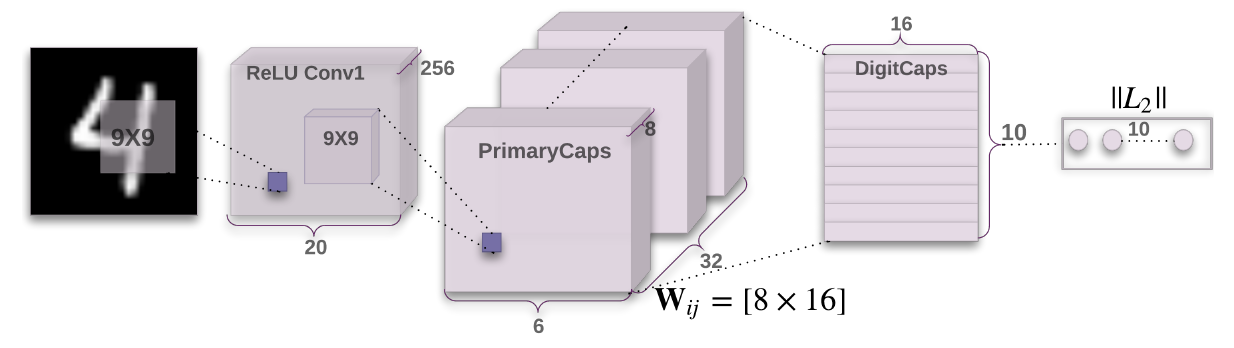
\includegraphics[width=1.0\textwidth]{capsnet.png}}
    \end{figure}
   
\begin{itemize}
	\item Shallow network with only two convolutional layers and one fully connected layer
	\item Routing is implemented only between PrimaryCaps and DigitCaps layers
\end{itemize}    
\end{frame}

\begin{frame}
\frametitle{Reconstruction as a regularization method}
\begin{figure}
	\subcapcentertrue
    \centering
    	\subfigure[Reconstruction from a capsule representation]
        {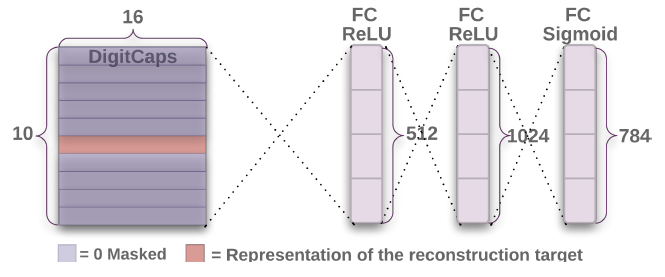
\includegraphics[width=0.6\textwidth]{reconstruction.png}}
    \end{figure}
   
An additional reconstruction loss is used to encourage the digit capsules to encode the instantiation parameters of the input digit. The output of the correct digit capsule is fed into a decoder consisting of 3 fully connected layers that model the pixel intensities. The objective function is the sum of squared differences between the outputs of the logistic units and the pixel intensities. This loss is scaled by 0.0005 so that it does not dominate the margin loss during training.
\end{frame}

\begin{frame}
\frametitle{Reconstruction results}
\begin{figure}
	\subcapcentertrue
    \centering
    	\subfigure[Digits reconstructed from the output of a capsule]
        {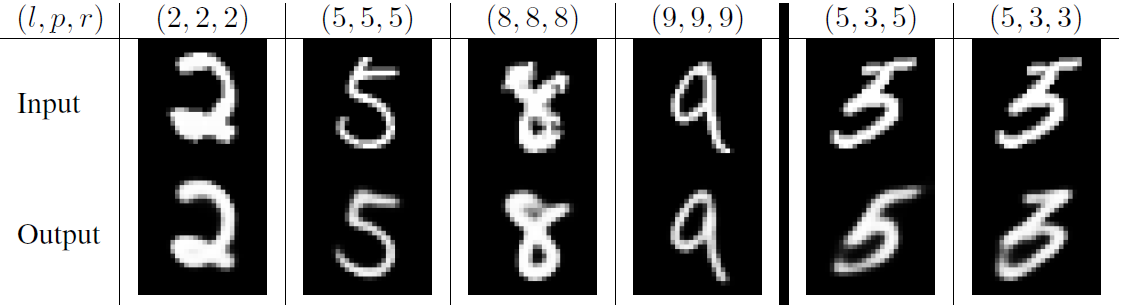
\includegraphics[width=1.0\textwidth]{reconstruction_results.png}}
    \end{figure}
\end{frame}

\begin{frame}
\frametitle{Results on MNIST}
\begin{figure}
	\subcapcentertrue
    \centering
    	\subfigure[Comparations between different network configurations and a CNN baseline]
        {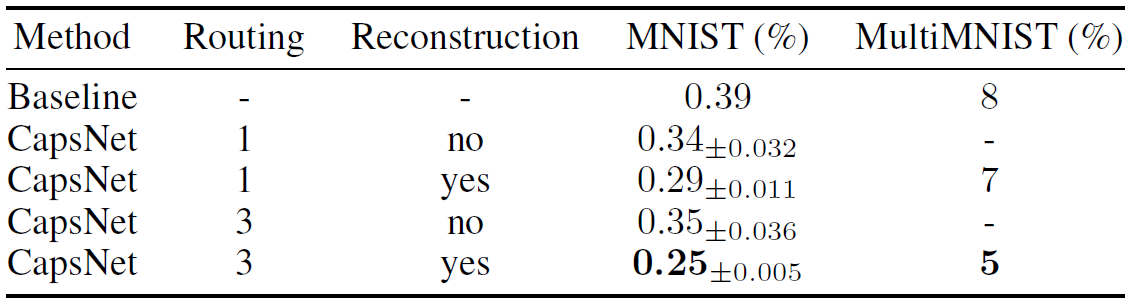
\includegraphics[width=0.9\textwidth]{comparation.png}}
    \end{figure}
The baseline is a standard CNN with three convolutional layers of 256, 256, 128 channels. Each has 5x5 kernels and stride of 1. The last convolutional layer is followed by two fully connected layers of size 328, 192. The last fully connected layers is connected with dropout to a 10 class softmax layer with cross entropy loss.
\end{frame}

\begin{frame}
\frametitle{What the individual dimensions of a capsule represent}
\begin{itemize}
	\item The dimensions of a digit capsule should learn to span the space of variations in the way digits of that class are instantiated (stroke thickness, skew and width)
	\item To see what the individual dimensions represent, a perturbed output vector can be fed to the decoder network to see how the perturbation affects the reconstruction
\end{itemize}
\begin{figure}
    \centering
    	\subfigure[Dimension peturbations]
        {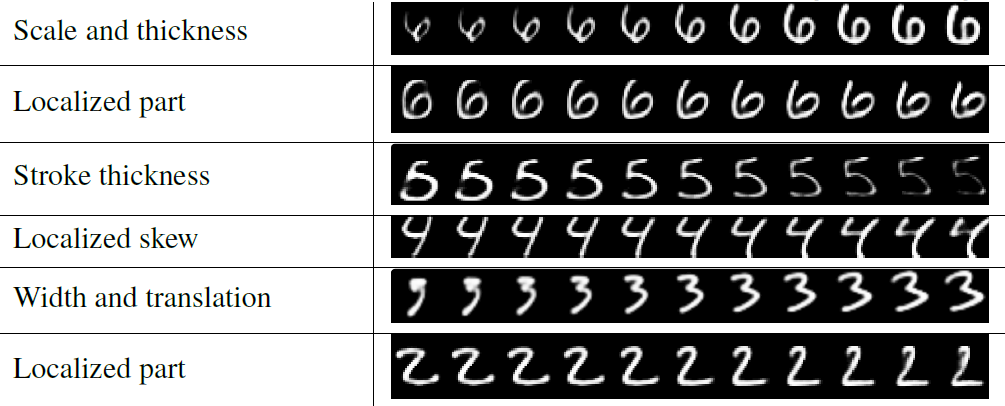
\includegraphics[width=0.75\textwidth]{perturbed.png}}
    \end{figure}
\end{frame}

\begin{frame}
\frametitle{Robustness to Affine Transformations}
\begin{itemize}
	\item Experiments show that each DigitCaps capsule learns a more robust representation for each class than a traditional convolutioanl network
	\item To test the robustness of CapsNet to affine transformations, a training was done on a padded and translated MNIST set, in which each example is an MNIST digit placed randomly on a black 				  background
	\item The network was tested on the affNIST \footcite{affNIST} data set, in which each example is an MNIST digit with a random small affine transformation
	\item CapsNet achieved 79\% accuracy, while a tranditional convolutional model with a similar number of parameters only 66\%
\end{itemize}
\end{frame}

\begin{frame}
\frametitle{Segmenting highly overlapping digits}
\begin{itemize}
	\item Dynamic routing can be viewed as a parallel attention mechanism that allows each capsule at one level to attend to some active capsules at the level below and to ignore others; This should allow the model to recognize multiple object in the image even if objects overlap
	\item To test this assumption, the MultiMNIST dataset was created by overlaying a digit on top of another from the same set, but different class, having 80\% average overlap
\end{itemize}
\end{frame}

\end{document}
